%\chapter{外文资料翻译}

\begin{translation}

\section{开放关系抽取:从监督数据到无监督数据的关系知识迁移}
\begin{center}
Ruidong Wu, Yuan Yao, Xu Han, 
\\
Ruobing Xie, Zhiyuan Liu, Fen Lin, Leyu Lin, Maosong Sun	
\end{center}


\subsection{引言}
关系提取(RE)的目的是从纯文本中提取两个实体之间的关系事实。例如,通过“宫崎骏是电影《风起云涌》的导演”这句话,我们可以提取出两个实体“宫崎骏”和“风起云涌”之间的关系“导演”。

最近,监督学习在关系抽取方面取得了巨大的成功。监督学习方法可以很有效地基于现有的标注数据学习到“关系-语义”模式,但这依赖于高质量的数据,然而数据的构建是非常耗费人力、物力的。为了降低监督的水平,已经有很多学者提出了几种半监督学习方法,包括bootstrapping、主动学习、标签传播等。Mintz提出了一种远程监督机制来自动生成训练数据。这种机制假设:如果两个实体在知识图谱中存在某种关系,那么所有包含这两个实体的句子都会表达这种关系。然而,这些方法都只能提取出已经在人类标注数据集或知识图谱中已经出现的预定义关系。这些方法很难覆盖开放域数据中的大量的新的关系事实。

开放式关系抽取(OpenRE)的目的是从开放域语料库中提取关系事实,其中关系的类型可能没有被预先定义。有一些工作旨在抽取具有新关系的三元组。Banko直接抽取句子中的单词或短语来表示新的关系类型。然而,有些关系不能用句子中的短语来明确表示,而且这也将导致相同关系的表示非常多样,无法对齐。 Yao将OpenRE建模为聚类任务,用于抽取具有新关系类型的三元组。然而,以往基于聚类的OpenRE方法大多是无监督的,不能有效地选择有意义的模式,丢弃不相关的信息。

本文提出了一种能够有效利用高质量的、标注了预定义关系的数据来实现开放关系抽取。由于在开放域中,预定义的关系和我们感兴趣的新关系之间存在着相当大的差距,因此这种方法是不能够被直接实现的。
因此,本文提出了关系孪生网络(Relational Siamese Networks, RSNs)来学习OpenRE中需要的可迁移的关系知识。具体而言,RSNs从标注了预定义关系的数据中学习如何度量关系事实的相似性,然后将该度量方法转移到未标注的句子上,以测量未标注句子的相似度,用于之后的开放关系聚类。图\ref{fig:appendix:openre-framework}中描述了本文模型框架的流程图。

\begin{figure*}
	\centering
	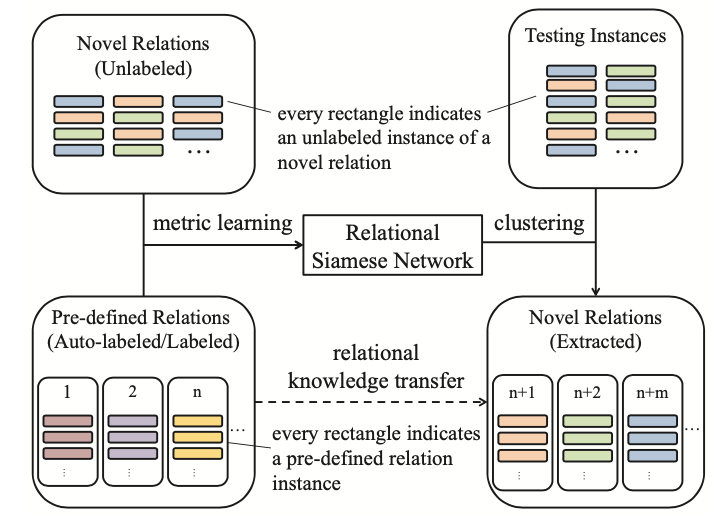
\includegraphics{appendix/openre-framework.png}
	\caption{本文模型框架的流程图。关系孪生网络从预定义关系的实例和未标注的新关系实例中学习,并在测试时对新关系的实例进行聚类。}
	\label{fig:appendix:openre-framework}
\end{figure*}

此外,RSNs也可以泛化到各种弱监督的场景。本文提出半监督关系孪生网络(Semi-supervised RSN)既可以从标注了预定义关系的有监督数据中学习,也可以从带有新关系的无监督数据中学习,而远程监督关系孪生网络(Distantly-supervised RSN)则可以从远程监督数据和无监督数据中学习。

本文在真实场景下的关系抽取数据集FewRel和FewRel-distant上进行实验,将数据集中的关系拆分成可见和不可见的关系集合,并在有监督、半监督和远程监督的场景中评估模型。结果表明,在不使用外部语言工具的情况下,本文模型在上述所有场景下都显著优于现有最先进的方法。总结而言,本文工作的主要贡献如下:
\begin{itemize}
	\item 本文提出了一种用于OpenRE的新的关系知识迁移框架RSN,这个模型可以有效地将现有的关系知识迁移到新关系数据上,并准确地抽取出新关系。同时,RSN是第一个在基于聚类的OpenRE任务中考虑知识迁移的模型。
	\item 本文进一步提出了能够在弱监督场景中学习的半监督关系孪生网络(Semi-supervised RSNs)和远程监督关系孪生网络(Distantly-supervised RSNs)。实验结果表明,与现有最先进的方法相比,这些RSN模型在F值方面都实现了显著的提升。
\end{itemize}

\subsection{相关工作}
\textbf{开放关系抽取。} 关系抽取是自然语言处理(Natural Language Processing, NLP)中一个非常重要的任务。传统的关系抽取方法主要聚焦于将关系事实分类为预定义的关系类型。Zeng利用卷积神经网络作为编码器,利用位置向量的帮助来构建句子表示。Lin通过实例级注意力机制,进一步提高了远程监督数据上的关系抽取性能。这些方法利用有监督或远程监督的数据来训练神经句子编码器,并取得了很好的效果。然而,这些方法不能处理在开放域中不断出现的新关系类型。

为了解决这个问题,最近很多学者投入了大量精力探索开放关系抽取,其目的是从无监督的开放域语料库中发现新的关系类型。OpenRE的方法大致可以分为两类:基于标记的方法和基于聚类的方法。基于标记的方法将OpenRE建模为一个序列标注问题,在无监督或有监督范式下,从句子中抽取出关系短语。然而,基于标记的方法往往会针对同一个关系类型提取出多个特定的关系短语,这也导致这种方法得到的结果在许多下游任务中无法直接运用。

相比之下,传统的基于聚类的OpenRE方法通过额外的语言学工具为关系实例提取出丰富的特征,并将特征聚类成新的关系类型。Marcheggiani提出了一种基于重构模型的离散状态变分自动编码器用于OpenRE。Elsahar利用聚类算法对语言特征进行聚类。在本文中,我们重点研究基于聚类的OpenRE方法,其优势在于发现高度可区分的新关系类型。

\textbf{少样本学习。} 少样本学习的目的是根据少量的标注数据对未标注数据进行分类。许多努力都致力于少样本图像分类和少样本关系分类。值得注意的是,Koch介绍了卷积孪生网络用于图像度量学习,这启发本文将关系的度量学习运用于OpenRE。

\textbf{半监督聚类。} 半监督聚类的目的是给定目标类别的部分实例来聚类相似的语义模式。不同的是,我们提出的半监督关系孪生网络只利用预定义的关系标签,不需要任何新关系的种子。


\subsection{方法}
本文提到的OpenRE框架主要由两个模块组成:关系相似度计算模块和关系聚类模块。在关系相似度计算方面,本文提出了关系孪生网络,该模块通过学习两个句子是否提到相同的关系来进行训练。为了利用大规模的无监督数据和远程监督数据,本文进一步提出了半监督关系孪生网络和远程监督关系孪生网络。最后,在关系聚类模块中,利用在关系相似度计算模块学习到的关系度量,本文使用分层聚类(HAC)和Louvain聚类算法来发现新关系类型。

\subsubsection{关系孪生网络(RSN)}
本文提出的关系孪生网络的架构如图\ref{fig:appendix:openre-rsn}所示。卷积神经网络模块将一对关系实例编码成向量,接着几个共享层计算它们的相似度。

\begin{figure*}
	\centering
	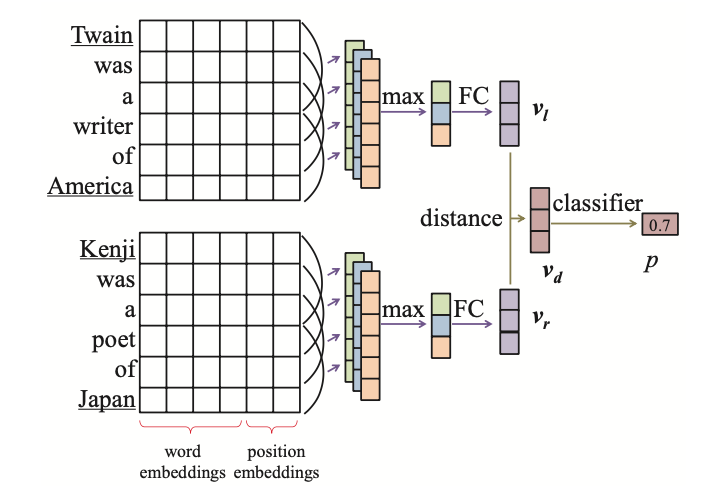
\includegraphics{appendix/openre-rsn.png}
	\caption{关系孪生网络的架构。输出为两个关系事实的相似度。}
	\label{fig:appendix:openre-rsn}
\end{figure*}

\textbf{句子编码器。}本文使用了一个卷积神经网络(Convolutional Neural Network, CNN)模块作为句子编码器。这个CNN模块包括一个词嵌入层、一个卷积层、一个最大池化层和一个全连接层。

词嵌入层将句子中的单词和实体 $e_{head}$ 和 $e_{tail}$ 的位置转化为预训练好的单词向量和随机初始化的位置向量。随后将这些向量拼接起来,形成一个向量序列。接下来,一个一维卷积层和一个最大池化层将向量序列转化为特征。最后,一个具有 $\text{Sigmoid}$ 作为激活函数的全连接层将句子特征映射成关系向量 $v$。总而言之,CNN模块将一个句子表示成一个向量 $v$:
\begin{equation}
	v = \text{CNN}(s)
\end{equation}
其中,$s$ 用来表示一个由句子 $s$ 和该句子中的两个实体 $e_{head}$ 和 $e_{tail}$ 组成的实例。并且,输入为一对关系实例,我们可以得到:
\begin{equation}
	v_l = \text{CNN}(s_l), v_r = \text{CNN}(s_r)
\end{equation}
其中,两个CNN模块共享参数,是相同的。

\textbf{相似度计算。}接下来,为了计算两个关系向量的相似度,我们先计算出两个关系向量的绝对距离,之后将其转化为实数相似度 $p \in [0,1]$。首先,距离层计算出两个向量的绝对距离:
\begin{equation}
	v_d = |v_l - v_r|
\end{equation}
接下来,一个分类层计算关系相似度的度量 $p$。这个分类层是一个输出为 $1$ 维且激活函数为 $\text{Sigmoid}$ 的全连接层:
\begin{equation}
	 p = \sigma(kv_d + b)
\end{equation}
其中 $\sigma$ 表示 $\text{Sigmoid}$ 函数,$k$ 和 $b$ 表示权重和偏差。

\textbf{交叉熵损失函数。}关系孪生网络的输出可以被看做两个关系实例表示两个不同关系的概率。因此,本文使用二值标签 $q$ 和二值交叉熵损失函数来训练关系孪生网络模型:
\begin{equation}
	\mathcal{L}_l = \mathbb{E}_{d_l~D_l}[q\text{ln}(p_\theta(d_l)) + (1-q)\text{ln}(1 - p_\theta(d_l))]
\end{equation}
其中,$\theta$ 指RSN的所有参数。

\subsubsection{半监督关系孪生网络(Semi-supervised RSN)}
为了能在开放域语料库中发现关系簇,模型不仅要从标注数据中学习,而且要捕捉到语义空间中的未标注数据的多样性,这样做对模型是有益的。为此,模型需要将决策边界推离高密度区域,这就是所谓的聚类假设。

本文尝试用几个附加的损失函数来实现这个目标。在下面的内容中,用 $D_l$ 表示带标注的训练数据集,用 $d_l$ 表示标注了关系的实例。同样,用 $D_u$ 表示不带标注的训练数据集,用 $d_u$ 表示没有标注关系的实例。

\textbf{条件熵损失函数。}在分类问题中,一个好的分类向量空间通常会在不同分类聚类之间预留较大的边缘距离,优化边缘距离可以成为帮助训练的很好的方法。然而,在聚类问题中,类型标签在训练过程中是不可用的。因此,为了在没有显式监督的情况下优化边缘距离,将数据点推离决策边界是一个有效的方法。直观地讲,当两个关系实例之间的距离相似度 $p$ 等于 $0.5$ 时,两个实例中至少有一个很接近关系簇之间的决策边界。因此,本文使用条件熵损失函数,该损失函数当 $p=0.5$ 时达到最大值,来惩罚数据点的近界分布。

\begin{equation}
	\mathcal{L}_u = \mathbb{E}_{d_u~D_u}[p_\theta(d_u)\text{ln}(p_\theta(d_u)) + (1-p_\theta(d_u))\text{ln}(1 - p_\theta(d_u))]
\end{equation}

\textbf{虚拟对抗损失函数。}条件熵最小化在理论上是有希望的,但在实践中却存在缺陷。由于神经网络具有很强的拟合能力,可能会学习到一个非常复杂的决策超平面,从而远离所有的训练样本,缺乏泛化性。为了解决这个问题,本文使用局部Lipschitz约束来平滑关系表示空间。

为了满足这个约束,我们在RSN的两个分支上都引入虚拟对抗训练。虚拟对抗训练可以通过数据点邻域搜索,对距离预测中最急剧的变化进行惩罚。对于标注数据,虚拟对抗损失函数为:
\begin{equation}
	\mathcal{L}_{v_l} = \mathbb{E}_{d_l~D_l}[\text{D}_\text{KL}(p_\theta(d_l)||p_\theta(d_l, t_1, t_2))]
\end{equation}
其中,$\text{D}_\text{KL}$ 指的是 KL 散度, $p_\theta(d_l, t_1, t_2)$ 指在对输入加入了 $t_1$ 和 $t_2$ 扰动后新的距离的估计。
具体来说, $t_1$ 和 $t_2$ 是在有限的长度下,使 $p_\theta(d_l)$ 和 $p_\theta(d_l, t_1, t_2)$ 之间的KL发散的最坏情况下的扰动。具体来说,我们首先在输入中加入一个随机噪声,并计算出原始输入与噪声输入的输出之间的KL散度的梯度。然后,我们将归一化梯度加到原始输入中,得到扰动输入。而对于未标注的数据,我们可以得到:
\begin{equation}
	\mathcal{L}_{v_u} = \mathbb{E}_{d_u~D_u}[\text{D}_\text{KL}(p_\theta(d_u)||p_\theta(d_u, t_1, t_2))]
\end{equation}
其中,扰动 $t_1$ 和 $t_2$ 是加在词向量上,而不是加在词本身上。

总结而言,本文使用了以下的损失函数来训练半监督关系孪生网络:
\begin{equation}
	\mathcal{L}_{all} = \mathcal{L}_l + \lambda_v\mathcal{L}_{vl} + \lambda_u(\mathcal{L}_u + \lambda_v\mathcal{L}_{vu})
\end{equation}
其中,$\lambda_v$ 和 $\lambda_u$ 是两个超参数。

\subsubsection{远程监督关系孪生网络(Distantly-supervised RSN)}
为了减少费时费力的人工标注工作,远程监督学习在关系抽取中引起了很多人的关注。本文提出了远程监督的关系孪生网络,它可以从远程监督的数据和无监督的数据中学习,实现关系知识迁移。具体来说,我们采用以下损失函数:
\begin{equation}
	\mathcal{L}_{all} = \mathcal{L}_l + \lambda_u(\mathcal{L}_u + \lambda_v\mathcal{L}_{vu})
\end{equation}
即,将自动标注的数据当做标注数据,但是在自动标注数据中去除了虚拟对抗损失函数。

移除虚拟对抗损失函数的原因很简单:对自动标注数据进行虚拟对抗性训练会放大虚假标签带来的噪声。事实上,实验结果证明,自动标注数据上的虚拟对抗会使模型的性能降低。

本文不使用更多的去噪方法,因为RSN在容忍噪声方面有一些固有的优势。首先,在训练过程中大量的负采样会压倒噪声。其次,在聚类过程中,预测一个新的关系聚类是基于关系密度较高的区域。因此,噪声产生的离群值不会对预测过程产生太大影响。

\subsubsection{开放关系聚类}
在训练了RSN之后,可以利用RSN计算出测试实例的相似度矩阵。利用这个矩阵,可以应用几种聚类方法来提取新的关系簇。

\textbf{层次聚类。} 本文采用的第一种聚类方法是层次聚类(Hierarchical Agglomerative Clustering,HAC)。HAC是一种自下而上的聚类算法。在开始时,每一个测试实例被视为一个类。在每一步中,它都会合并两个最接近的簇。有许多标准来评估两个簇之间的距离。本文采用的是完全联系标准,它对极端实例更稳定。

然而,HAC有一个显著的缺陷:它需要指定聚类后类的数量。一个潜在的解决方案是根据经验距离阈值停止聚类,但很难确定这样的阈值。这个问题导致本文考虑另一种聚类算法Louvain算法。

\textbf{Louvain聚类算法。}Louvain是一种基于图的聚类算法,传统上用于社群检测。为了构造图,本文使用RSN输出的二进制近似,$0$ 表示两个节点之间有一条边。Louvain的优点是,它不需要事先确定聚类数量。它将通过优化社区的模块度,自动找到合适大小的簇。根据本文进行的实验,Louvain的性能比HAC更好。

在运行后,Louvain可能会产生一些单子簇,其中的实例很少。把这些簇称为新的关系是不合适的,所以我们把这些实例标注上和它们最接近的邻居的相同的标签。

最后,我们想解释一下为什么不使用其他一些常用的聚类方法,如K-Means、Mean-Shift等方法:这些方法在聚类过程中仅仅通过计算几个向量的平均值来计算中心点。但是,我们的模型中的关系向量是高维的,且RSN所描述的距离度量是非线性的。因此,单纯地用向量的平均化来计算中心点是不合适的。


\subsection{实验分析}
在本节中,我们在真实世界的关系抽取数据集开展了几个实验,展示了本文模型的有效性,并给出了详细的分析,以显示模型优势。

\subsubsection{数据集}
在实验中,我们使用FewRel作为我们的第一个数据集。FewRel是一个手工标注的数据集,包含 $80$ 种类型的关系,每个关系有 $700$ 个实例。FewRel的一个优点是每个实例都包含一个唯一的实体对,所以关系抽取模型无法通过简单记忆实体的方式来判断关系。

我们将包含 $64$ 个关系的FewRel的原始训练集作为预先定义好的关系的标注集,将包含 $16$ 个新关系的FewRel的原始验证集作为提取新关系的未标注集。然后,我们从未标注集中随机选择 $1600$ 个实例作为测试集,其余有标签的和无标签的实例作为训练集。

我们使用的第二个数据集是FewRel-distant,它包含了FewRel作者在手工标注之前获得的远程监督数据。我们按照FewRel的拆分方式,得到自动标注的训练集和未标注的训练集。为了评估,我们使用了FewRel的人工标注的测试集,有 $1,600$ 个实例。在FewRel-distant的训练集中删除在测试集中出现的实例。最后,自动标记的训练集包含 $323,549$ 个关系实例,而未标记的训练集包含 $60,581$ 个实例。

之前OpenRE的一个工作在一个名为NYT-FB的非公开数据集上进行了测试。然而,与FewRel-distant相比,这个数据集有以下缺点:首先,NYT-FB的测试集是远距离监督的,对于实例级的关系抽取来说,它的测试集是嘈杂的;此外,NTY-FB中的实例经常共享实体对,这使得关系聚类更加容易。因此,我们认为FewRel-distant上的结果对于Distantly-supervised OpenRE来说是足够有说服力的。

\subsubsection{实现细节}
\textbf{数据采样。} RSN的输入是一对关系实例。对于无标注数据集,唯一可能的采样方法是随机选择两个实例。对于有标签的数据集,随机选择会导致过多的不同关系实例对,将对RSN造成严重的偏差。为了解决这个问题,我们使用向下采样的方法。在我们的实验中,我们将每批有标签数据中的具有相同关系的实例对的百分数固定为 $6\%$。

\textbf{超参设置。} 本文使用了预训练的 $50$ 维的Glove词向量。对于位置向量,本文使用了随机初始化的 $5$ 维的位置向量。在训练时,所有的词向量、位置向量都是可训练的。对于神经网络,卷积神经网络中的特征维度为 $230$。最大池化层之后的激活函数为ReLU,全连接层之后的激活函数为Sigmoid。除此之外,本文在CNN模块使用了两种正则化方法。本文在词向量层后使用了丢失层,丢失率为 $0.2$。我们在卷积层和全连接层上使用了 $L2$ 正则化项。

同时,主要的超参数是在验证集上使用了网格搜索后根据模型效果挑选的。其中,验证集包含了从未标注集合中随机挑选的 $1000$ 个样例,并且与测试集中的样例没有重合。

\subsubsection{开放关系抽取的实验结果}
这一节通过与其他的最先进的算法进行比较,展示了本文提出的关系孪生网络的有效性。同时,作者也开展了消融实验来详细分析在半监督关系孪生网络及远程监督关系孪生网络中提出的不同的机制给模型带来的增益。

\textbf{基线模型。} 传统的基于聚类的开放关系抽取的方法通常通过聚类句子的语言特征或引入重构造限制来实现。为了展现关系孪生网络的有效性,本文将模型与以下两个最先进的模型进行比较:
\begin{itemize}
	\item 带有重新加权的词向量的层次聚类(re-weighted word embeddings HAC, RW-HAC):RW-HAC是目前在开放关系抽取上最先进的特征聚类模型。这个模型首先抽取实体的知识库类型及命名实体识别标签和重新加权的词向量,接着使用主成分分析法来减少特征维度,最后使用层次聚类算法来对降维后的特征进行聚类。
	\item 离散变分自动编码器(discrete-state variational autoencoder, VAE):VAE是目前在开放关系抽取任务上基于重构造的最先进的模型,它能够利用未标注数据。该模型根据实体对及预测关系类型来重构造实体来优化关系分类器。模型利用了丰富的特征:实体单词、上下文单词、依赖路径和上下文的词性标签来预测关系类型。
\end{itemize}

RW-HAC和VAE都依赖与外部语言工具来实现从文本中抽取丰富的特征。具体来说,首先将实体与维基数据中实体对齐,并获得它们的实体类型。接下来,我们用词性标注工具、命名实体识别工具、以及Stanford CoreNLP的句法依存工具对句子进行预处理。值得注意的是,这些特征只被基线模型使用。相比之下,本文的模型只使用句子和实体对作为输入。

\textbf{评测。} 在模型评测中,我们使用B3度量作为评测函数。B3度量是平衡聚类任务的精度和召回的标准度量,在之前的开放关系抽取工作中经常被使用。具体来说,这是使用F1度量,即精度和召回的谐波均值。

首先,本文报告使用了不同聚类方法的有监督关系孪生网络的效果。具体来说,$\text{SN}$ 表示原始关系孪生网络结构,$\text{HAC}$ 和 $\text{L}$ 表示HAC和Louvain聚类,Louvain聚类在第3.3节中介绍过。结果表明,Louvain的表现优于HAC,所以在下面的研究中,我们重点介绍使用Louvain聚类。

接下来,对于半监督的RSN和远程监督的RSN,我们对不同的机制进行不同的组合,以验证各部分的对比。(+C)表示该模型是用条件熵最小化的方法来驱动,而(+V)表示该模型是用虚拟对抗训练的方法来驱动。



\begin{table}[]
\centering
\begin{tabular}{lllllll}
\toprule
         & \multicolumn{3}{l}{FewRel} & \multicolumn{3}{l}{FewRel-distant} \\
Approach & P     & R     & $F_1$   & P        & R       & $F_1$      \\ \midrule
VAE      & 17.9  & 69.7  &  28.5   &  17.9    & 69.7    &  28.5      \\
RW-HAC   & 31.8  & 46.0  &  37.6   &  31.8    & 46.0    &  37.6      \\ \midrule
SN-HAC   & 36.2  & 53.3  &  43.1   &  34.5    & 53.3    &  41.5      \\
SN-L     & 36.5  & 69.2  &  47.8   &  34.6    & 59.8    &  43.9      \\
SN-L+V   & 46.1  & 77.3  &  57.8   &  40.7    & 52.4    &  45.8      \\
SN-L+C   & 47.1  & \textbf{78.1}  &  58.8   &  \textbf{42.3}    & 66.0    & 51.5       \\
SN-L+CV  & \textbf{48.9}  &   77.5  & \textbf{59.9}  &  40.8   & \textbf{74.0} & \textbf{52.6}           \\ \bottomrule
\end{tabular}
\caption{不同模型的准确率、召回率和F1的值。开头两个模型是基线模型。接下来的五个模型是本文提出的模型的变种。}
\label{appendix:openre:result}
\end{table}

\textbf{实验结果分析。} 表\ref{appendix:openre:result}展示了实验结果。从中可以发现以下结论:
\begin{itemize}
	\item 关系孪生网络模型在准确度、召回率和F1值上均优于所有的基准模型,其中弱监督的关系孪生网络(SN-L+CV)达到了最先进的性能。这表明关系孪生网络能够理解句子中的新关系的语义。
	\item 有监督或远程监督的关系表示提高了聚类的性能。与RW-HAC相比,SN-HAC由于其有监督的关系表示和相似度量的关系表示,获得了更好的聚类结果。具体来说,无监督基线模型主要使用稀疏的独热特征。RW-HAC使用词嵌入,但以规则为基础的方式进行整合。相比之下,RSN使用分布式特征表示法,可以根据监督信息优化信息整合过程。
	\item 从SN-HAC和SN-L的比较来看,Louvain在RSN模型的聚类方面优于HAC。一种解释是本文的模型没有对关系向量的先验分布进行额外的约束,因此关系簇可能具有奇异的形状,违反了HAC的假设。此外,当关系表示不够可区分时,强迫HAC寻找细粒度的类别可能会损害找回,而对精度的贡献最小。在实践中,我们确实发现SN-L提取的关系数总是小于真实的16。
	\item SN-L+V和SN-L+C都是通过进一步利用无监督数据来提高有监督或远监督的RSN的性能。这两种半监督的方法都通过提高精度和召回率,为F1得分带来了显著的改善,而将两者结合起来,可以进一步提高F1得分。
	\item 一个有趣的观察结果是,SN-L+V在FewRel-distant上的表现并没有显著优于SN-L。这可能是因为在噪声数据上的虚拟对抗训练可能会放大噪声。在进一步的实验中,我们仅在未标记的集上进行虚拟对抗训练,观察到在F1上的改进,SN-L+V从45.8\%提高到49.2\%,SN-L+CV从52.0\%提高到52.6\%,这证明了这个猜想。
\end{itemize}


\subsubsection{预定义关系的多样性对模型泛化能力的影响}
\begin{figure*}
	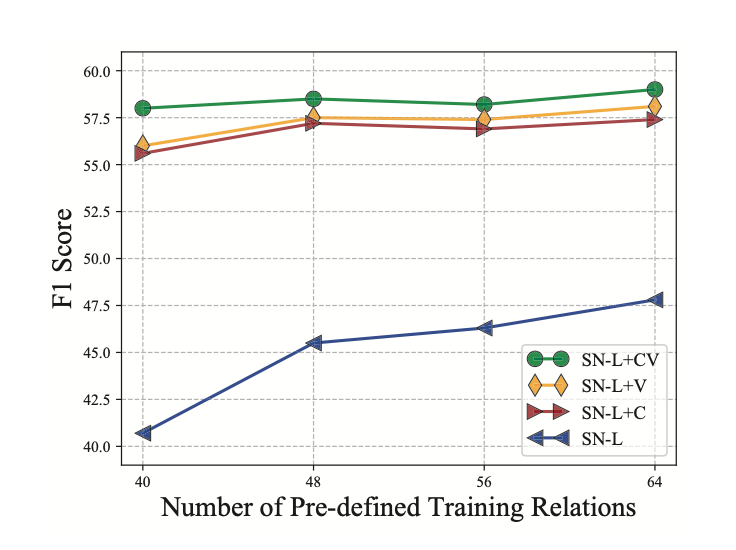
\includegraphics{appendix/openre-relationnum.png}
	\caption{训练集中预定义关系数量与聚类结果的对应图}
	\label{appendix:figure:openre-relationnum}
\end{figure*}

在这一小节中,我们主要分析预定义关系多样性的影响,即标注训练集中的关系数量。为了研究这种影响,我们使用FewRel进行评估,将标注训练集中的关系数从 $40$ 个变为 $64$ 个,同时将标签化实例的总数固定为$25,000$ 个,并将聚类结果报告在图\ref{appendix:figure:openre-relationnum}中。

根据图\ref{appendix:figure:openre-relationnum},可以得出几个结论。首先,丰富的标签关系确实提高了我们模型的性能,尤其是RSN。在64个关系上训练的模型的性能要比在40个关系上不断训练的模型要好。其次,虽然有监督的RSN的性能对预设的关系多样性非常敏感,但它的半有监督的对应模型受关系数限制的影响要小得多。这一现象表明,半监督的RSN在从未标记的新颖关系数据中学习成功,并且对新颖关系的通用性更强。


\subsubsection{关系表示可视化}
\begin{figure*}
	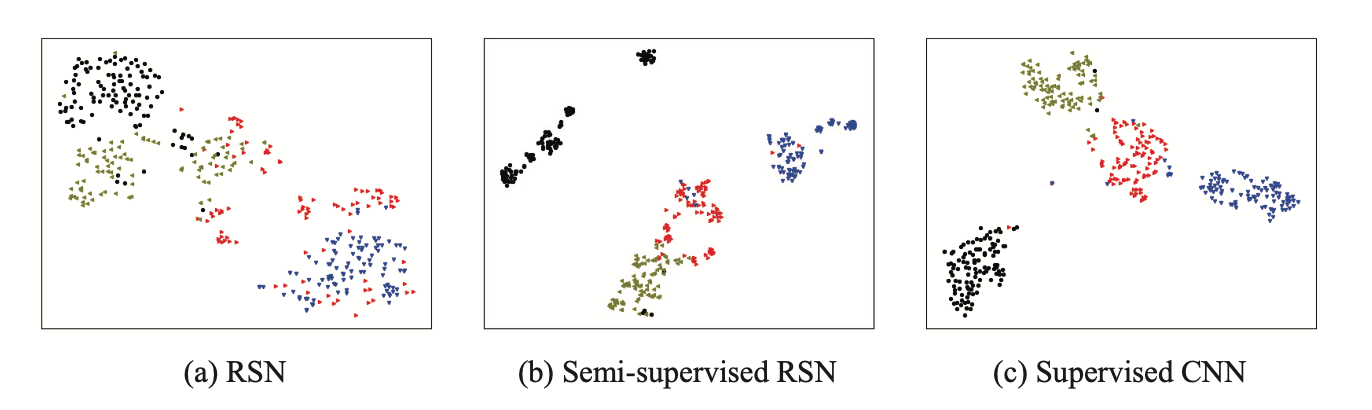
\includegraphics[width=\linewidth]{appendix/openre-visual.png}
	\caption{CNN模块输出的向量的t-SNE可视化。(a)关系孪生网络;(b)半监督关系孪生网络;(c)经典的有监督关系抽取模型。所有的图都显示了4种新型关系的402个实例的聚类结果。}
	\label{appendix:figure:openre-visual}
\end{figure*}

为了直观地评估RSN和半监督的RSN的知识转移效果,我们在图\ref{appendix:figure:openre-visual}中用t-SNE的CNN编码器最后一层的输出向量直观地展示了它们的关系知识表示空间。我们还与在 $9,600$ 个被标记的新颖关系实例上训练了有监督的CNN进行比较,提出了最优的关系知识表示空间。在每张图中,我们绘制了测试集中4种随机选择的关系类型的402个关系实例,并用颜色表示不同关系的数据。

从图\ref{appendix:figure:openre-visual}中可以看出,RSN能够大致区分不同的关系,而半监督的RSN在训练过程中通过优化潜在的关系簇之间的边界,进一步促进了知识转移。因此,半监督RSN能够提取出更多可区分的新奇关系,获得了与有监督CNN相当的关系知识表示能力。

\subsection{结论及未来工作}
本文提出了一个新的模型——关系孪生网络(RSN),用于开放关系抽取。与传统的无监督模型不同的是,我们的模型可以从预设关系的有监督/有监督的数据中学习度量关系的相似度,也可以从新颖关系的无监督数据中学习度量关系的相似度。我们的模型主要有两个创新点。首先,我们提出了用RSN结构来迁移关系相似度知识。就我们所知,我们是第一个提出了OpenRE的知识迁移。第二,我们提出了半监督/远距离监督的RSN,进一步进行半监督和远距离监督的迁移学习。实验表明,我们的模型显著超越了传统的OpenRE模型,实现了新的最先进的性能。

对于未来的研究,我们计划从以下几个方向进行探索。(1)除了CNN之外,还有一些其他流行的句子编码器结构,如分片卷积神经网络(PCNN)、长短时记忆神经网络(LSTM)等用于RE的句子编码器结构。在未来,我们可以在我们的模型中尝试不同的句子编码器。2)如上所述,我们的模型具有发现关系的层次结构的潜在能力。在未来,我们将尝试通过额外的实验来探索这种应用。

\nocite{wu2019open}
\bibliographystyle{thuthesis-bachelor}     % 本科生参考文献的著录格式
\bibliography{ref/refs}

\end{translation}


